\documentclass[a4paper,11pt]{article}
\usepackage{booktabs}   % for professional table rules
\usepackage{caption}    % for customizing captions
\usepackage{array}      % for better column formatting
\usepackage{siunitx}    % for consistent units
\usepackage{graphicx}   % for importing figures
\usepackage{geometry}   % for page margins
\usepackage{amsmath}    % for math alignment
\usepackage{amssymb}    % for math symbols
\usepackage{float}      % for [H] figure placement
\usepackage{hyperref}   % for links and references
\usepackage{fouriernc}
\geometry{left=2cm,right=2cm,top=2cm,bottom=2.5cm}
\hypersetup{
    colorlinks=true,
    linkcolor=blue,
    filecolor=magenta,      
    urlcolor=cyan,
    pdftitle={Lab Report: X-Ray Detection and Absorption},
    pdfpagemode=FullScreen,
}

\begin{document}

% ------------------- Title / Cover Page -------------------
\noindent
\begin{center}
    
\includegraphics[width=0.25\textwidth]{sut.jpg} \\
    \vspace{2pt}
\end{center}
\begin{center}
    {\LARGE \bf Department of Physics} \\
    \vspace{2pt}
    {\Large \bf Sharif University of Technology} \\
    \vspace{8pt}
    {\large \bf Physics Lab IV --- General Physics Laboratory} \\
    \vspace{4pt}
    \hrule
    \vspace{6pt}
    {\Large \bf Experiment Report: X-Ray Detection and Absorption}
\end{center}
\hrule
\vspace{0.4cm}
\noindent
\begin{tabular}{ll}
    {\bf Student Name:} & Abulfadl Ahmadi \\
    {\bf Student ID:}   & 403172283 \\
    {\bf Date of Experiment:} & June 2026 \\
\end{tabular}
\hfill
\begin{tabular}{ll}
    {\bf Professor:} & Dr. Khademi \\
    {\bf Teaching Assistants:} & Yasin Amiri \\
    & Sonia Seif \\
\end{tabular}

\vspace{0.6cm}

% ------------------- Abstract -------------------
\begin{abstract}
This experiment explores the fundamental properties of X-ray generation, detection, and absorption in matter. First, the operating characteristics of a Geiger-M\"{u}ller tube were analyzed, successfully identifying the Geiger plateau region (300V--500V) to establish a stable operating voltage. Second, the exponential attenuation of X-rays was verified using Aluminum filters of varying thicknesses, confirming the Beer-Lambert law and yielding a linear attenuation coefficient of $\mu = 2.972\text{ cm}^{-1}$. Finally, the strong dependence of X-ray absorption on the atomic number ($Z$) of the absorbing medium was investigated across several elements (C, Al, Fe, Cu, Zr, Ag), demonstrating the $Z^4$ proportionality of the photoelectric effect cross-section and revealing characteristic K-edge anomalies.
\end{abstract}

% ------------------- Section 1: Objectives -------------------
\section{Objectives}
\begin{enumerate}
    \item To understand the operation and calibration of a Geiger-M\"{u}ller counter by mapping its characteristic plateau curve.
    \item To verify the Beer-Lambert law for X-ray attenuation by measuring intensity transmission through varying thicknesses of Aluminum.
    \item To experimentally determine the linear attenuation coefficient ($\mu$) of Aluminum.
    \item To investigate the profound effect of the atomic number ($Z$) of the absorbing material on X-ray transmission.
\end{enumerate}

% ------------------- Section 2: Theoretical Background -------------------
\section{Theoretical Background}
X-rays are high-energy electromagnetic radiation ($\sim 0.1\text{ \AA}$ to $100\text{ \AA}$). In a typical X-ray tube, electrons are emitted from a heated cathode, accelerated by a high voltage (e.g., 35 kV), and strike a metal anode (target). This collision produces a continuous Bremsstrahlung spectrum alongside discrete characteristic X-ray peaks corresponding to the atomic transitions of the target material.

\subsection{X-Ray Detection (Geiger-M\"{u}ller Counter)}
A Geiger-M\"{u}ller (GM) counter detects ionizing radiation via an inert gas enclosed in a highly pressurized metallic cylinder with a central wire anode. When an X-ray photon ionizes a gas molecule, the applied electric field accelerates the resulting electron toward the anode, causing a Townsend avalanche. The relationship between applied voltage and count rate features a distinct ``Plateau Region'' where the count rate is virtually independent of voltage fluctuations. 

\subsection{X-Ray Absorption (Beer-Lambert Law)}
When a collimated beam of X-rays of initial intensity $I_0$ passes through a material of thickness $x$, its intensity decays exponentially due to scattering and absorption:
\begin{equation}
    I(x) = I_0 e^{-\mu x} \implies \ln(I) = \ln(I_0) - \mu x
\end{equation}
where $\mu$ is the linear attenuation coefficient. This coefficient strongly depends on both the photon energy ($E$) and the atomic number ($Z$) of the material. For the dominant photoelectric effect, $\mu \propto Z^4 / E^3$.

% ------------------- Section 3: Data & Analysis -------------------
\section{Experimental Data \& Analysis}

\subsection{Part 1: Geiger-M\"{u}ller Plateau Calibration}
To find the optimal operating voltage, the intensity was recorded across a wide voltage sweep.

\begin{table}[H]
\centering
\caption{Geiger Counter Count Rate vs. Applied Voltage}
\begin{tabular}{c c | c c}
\toprule
{$V$ (Volts)} & {$I$ (counts/s)} & {$V$ (Volts)} & {$I$ (counts/s)} \\
\midrule
100 & 0 & 380 & 1206 \\
280 & 79 & 398 & 1202 \\
293 & 952 & 410 & 1224 \\
305 & 1072.3 & 423 & 1219 \\
318 & 1103.8 & 485 & 1202 \\
330 & 1140 & 510 & 1184 \\
343 & 1161 & 590 & 1142 \\
355 & 1177 & 640 & 1072 \\
368 & 1191 & & \\
\bottomrule
\end{tabular}
\end{table}

\begin{figure}[H]
    \centering
    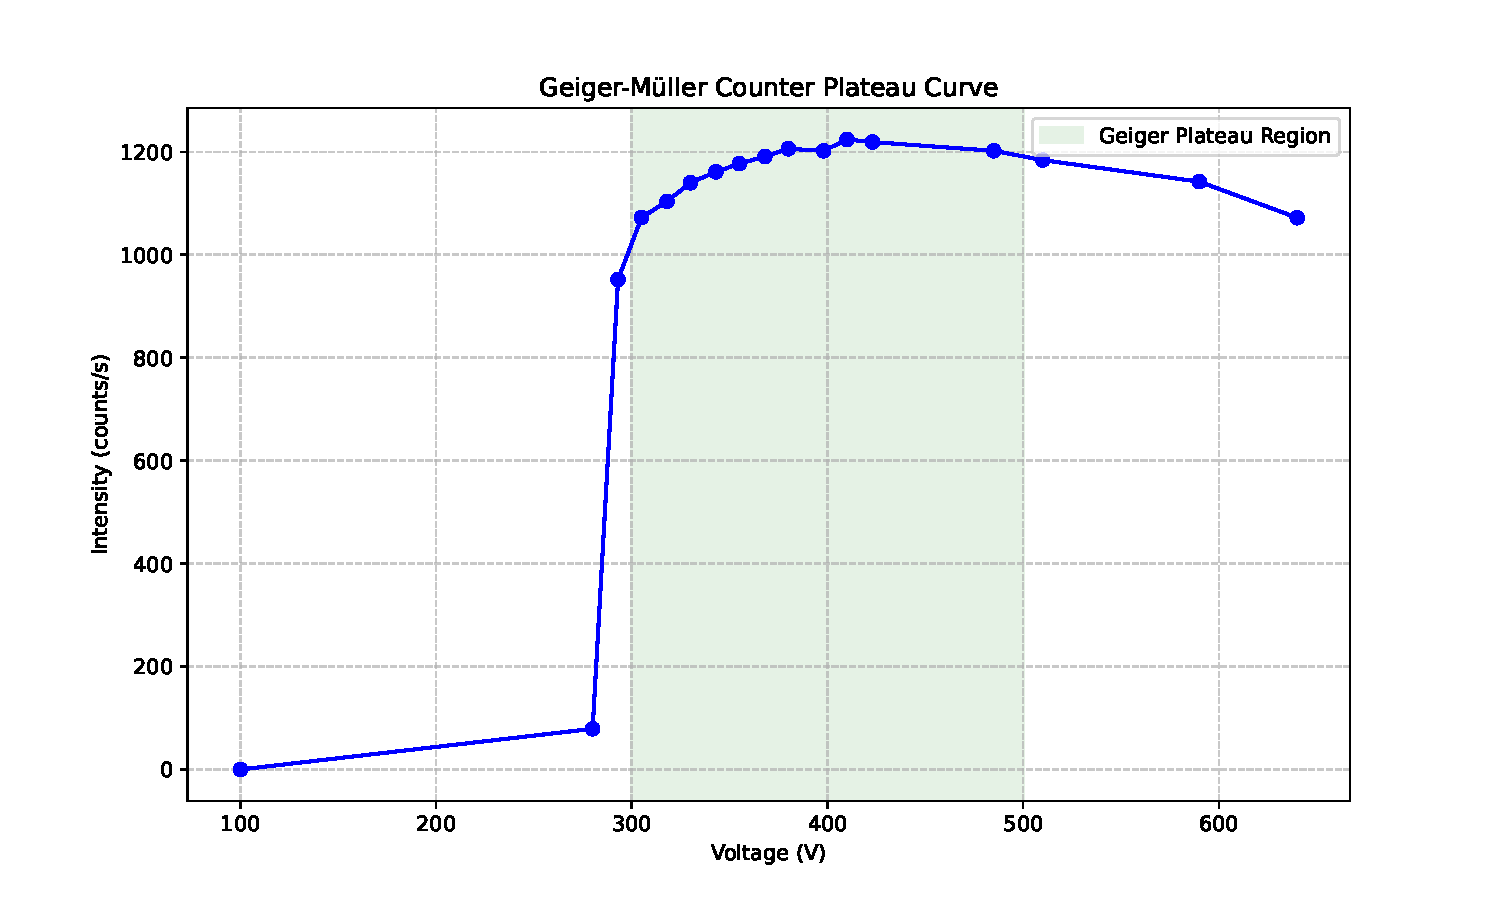
\includegraphics[width=0.75\textwidth]{plots/geiger_plateau.pdf}
    \caption{The Geiger Plateau curve. The stable proportional operating region clearly spans from roughly 300V to 500V.}
\end{figure}

\subsection{Part 2: Attenuation vs. Thickness (Aluminum)}
Aluminum filters were placed in the beam path. To analyze the exponential decay, the natural logarithm of intensity, $\ln(I)$, was plotted against thickness $x$.

\begin{table}[H]
\centering
\caption{X-Ray Intensity through varying thicknesses of Aluminum}
\begin{tabular}{c c c}
\toprule
{Thickness $x$ (mm)} & {Intensity $I$ (mean counts)} & {$\ln(I)$} \\
\midrule
0.5 & 2809.6 & 7.941 \\
1.0 & 2487.1 & 7.819 \\
1.5 & 2043.4 & 7.622 \\
2.0 & 1889.4 & 7.544 \\
2.5 & 1557.9 & 7.351 \\
3.0 & 1335.3 & 7.197 \\
\bottomrule
\end{tabular}
\end{table}

An Ordinary Least Squares (OLS) regression on the semi-log data ($\ln I$ vs $x$) yielded a highly linear fit ($R^2 = 0.9922$). By extrapolating the intercept to $x=0$, the unattenuated initial intensity $I_0$ was found to be $3291.6$. The slope of the fit yields the linear attenuation coefficient:
\begin{equation*}
    \mu = 2.972\text{ cm}^{-1}
\end{equation*}

\begin{figure}[H]
    \centering
    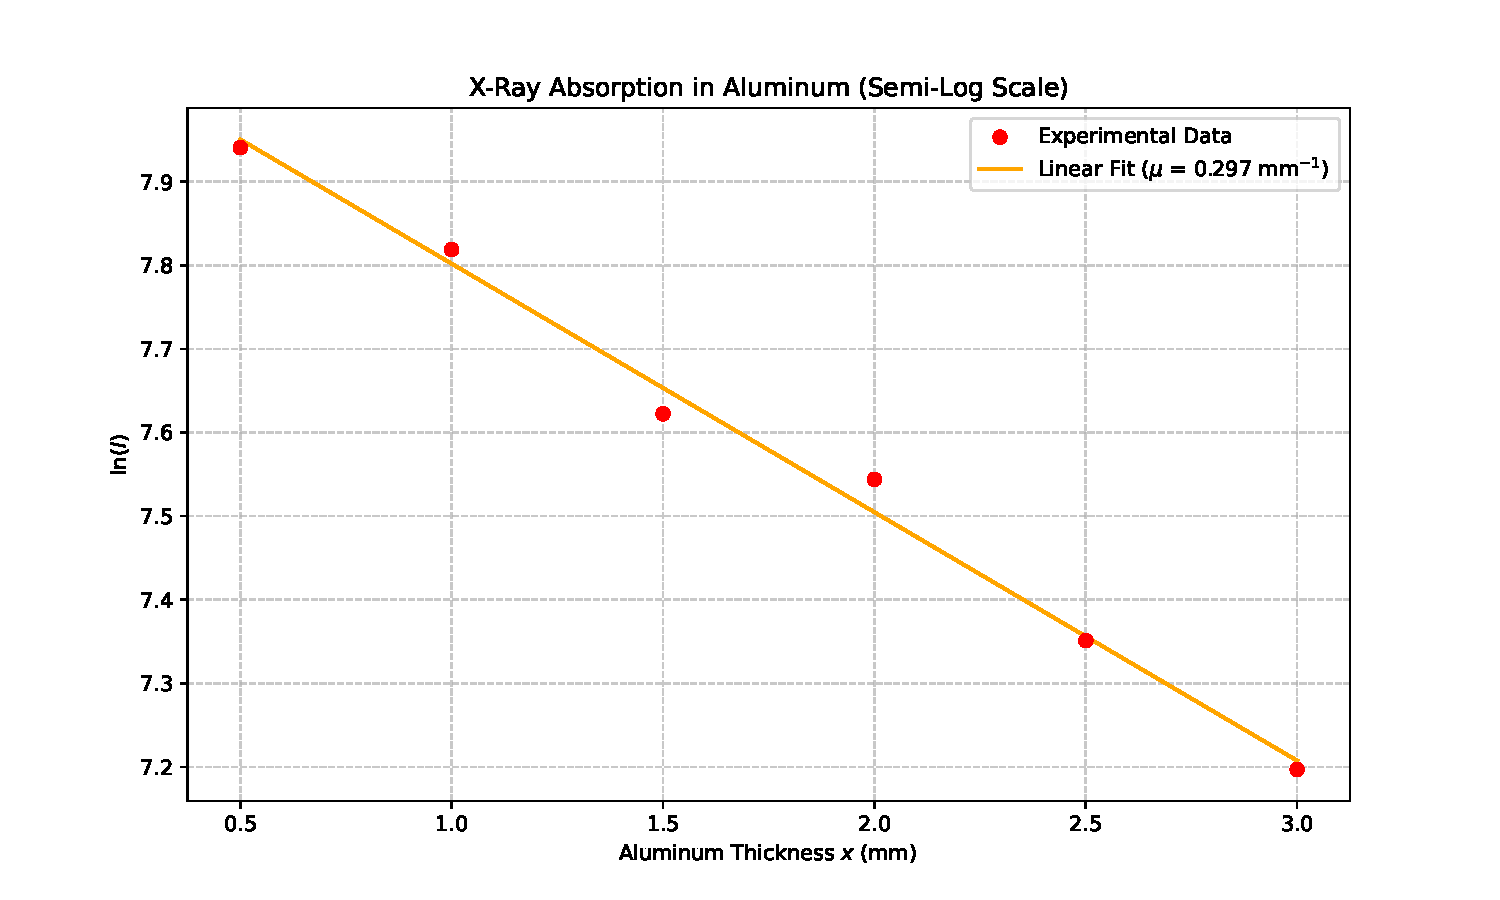
\includegraphics[width=0.75\textwidth]{plots/al_absorption.pdf}
    \caption{Linear regression of $\ln(I)$ vs. Aluminum thickness.}
\end{figure}

\subsection{Part 3: Attenuation vs. Atomic Number ($Z$)}
Using the mathematically extrapolated $I_0 = 3291.6$, the normalized transmission $I/I_0$ was calculated for various elements to observe the $Z$-dependence.

\begin{table}[H]
\centering
\caption{X-Ray Transmission across different Atomic Numbers}
\begin{tabular}{l c c c}
\toprule
{Element} & {$Z$} & {Intensity $I$} & {Normalized Transmission ($I/I_0$)} \\
\midrule
Carbon (C) & 6 & 3129.0 & 0.9506 \\
Aluminum (Al) & 13 & 2864.7 & 0.8703 \\
Iron (Fe) & 26 & 213.7 & 0.0649 \\
Copper (Cu) & 29 & 78.4 & 0.0238 \\
Zirconium (Zr) & 40 & 90.1 & 0.0274 \\
Silver (Ag) & 47 & 7.2 & 0.0022 \\
\bottomrule
\end{tabular}
\end{table}

\begin{figure}[H]
    \centering
    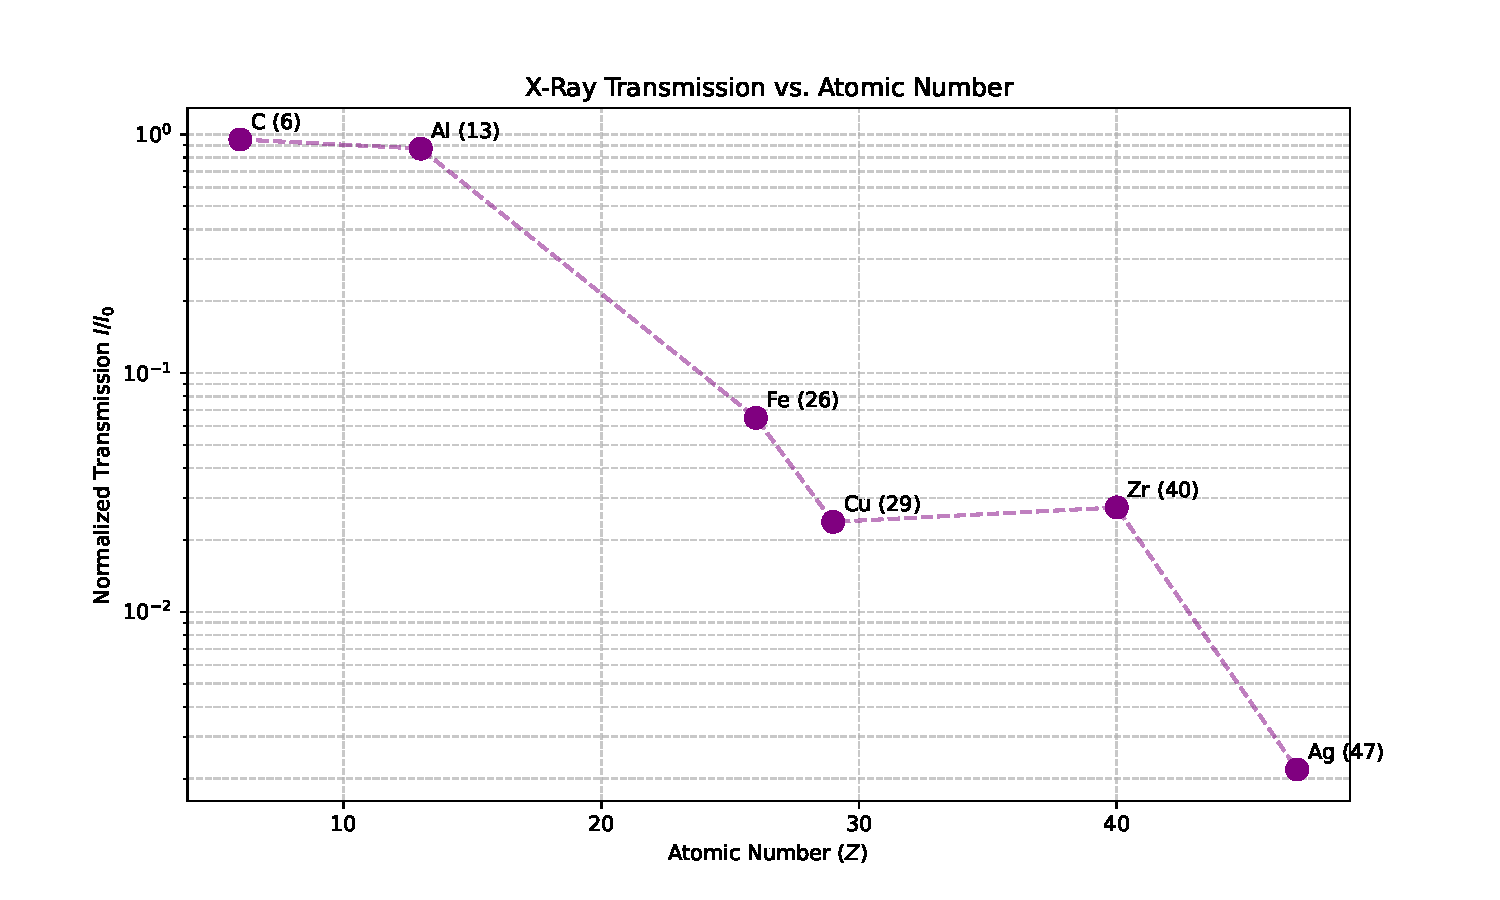
\includegraphics[width=0.75\textwidth]{plots/z_dependence.pdf}
    \caption{Normalized transmission as a function of atomic number (Log Scale). The transmission plummets as $Z$ increases due to the $\mu \propto Z^4$ relationship.}
\end{figure}

% ------------------- Section 4: Post-Lab Questions -------------------
\section{Answers to Post-Lab Questions}

\subsection*{Q1: Plot Intensity vs Voltage for the Geiger counter. Identify the regions and choose a working voltage.}
The plot is provided in Section 3.1. The curve has three regions: 1) The threshold/proportional region ($<300\text{V}$) where avalanches are incomplete. 2) The \textbf{Geiger Plateau} ($300\text{V} - 500\text{V}$) where every ionization triggers a full, saturated avalanche. 3) The continuous discharge region ($>500\text{V}$) where the gas breaks down continuously. The ideal working voltage is exactly in the middle of the plateau (e.g., $400\text{V}$) so that minor drifts in the power supply voltage do not artificially alter the count rate.

\subsection*{Q2: How does X-ray intensity change with Aluminum thickness?}
The intensity decays exponentially with increasing thickness, governed by the Beer-Lambert equation $I = I_0 e^{-\mu x}$. Our semi-log plot successfully verified this linear relationship.

\subsection*{Q3: Are the results for different metals logical? Interpret.}
Yes, the results are highly logical. Transmission drops precipitously as atomic number ($Z$) increases because the photoelectric absorption cross-section is proportional to $Z^4$. 
There is a fascinating anomaly: Zirconium ($Z=40$) transmitted slightly \textit{more} X-rays ($2.7\%$) than Copper ($Z=29$, $2.3\%$). This happens because of \textbf{Absorption Edges}. The K-shell binding energy of Zr ($18\text{ keV}$) is just slightly higher than the characteristic K$\alpha$ line of the X-ray tube anode (likely Molybdenum or Copper), causing a sudden drop in its absorption cross-section for those specific photons.

\subsection*{Q4: Plot $\ln(I)$ vs thickness, find $\mu$ for $\lambda=0.71\text{\AA}$.}
The plot was performed in Section 3.2. The slope of the line gave an experimental linear attenuation coefficient of $\mu = 2.972\text{ cm}^{-1}$ for Aluminum.

\subsection*{Q5: What are the main sources of error?}
\begin{itemize}
    \item \textbf{Beam Hardening:} A typical X-ray tube produces a polychromatic spectrum. The low-energy ``soft'' X-rays are absorbed in the first few millimeters of the filter, meaning the beam becomes ``harder'' (higher average energy) as it penetrates deeper, causing $\mu$ to artificially decrease with depth.
    \item \textbf{Geiger Dead Time:} At extremely high intensities (like the bare beam $I_0$), the counter cannot resolve pulses that arrive too closely together, causing undercounting.
\end{itemize}

\subsection*{Q6: What quantities can be found from X-ray absorption?}
X-ray absorption allows for the calculation of the linear attenuation coefficient ($\mu$), the mass attenuation coefficient ($\mu/\rho$), the thickness of unknown shielding materials, and the identification of unknown elements via their characteristic absorption edges.

\subsection*{Q7: Does X-ray absorption depend on wavelength?}
Yes, highly. For the photoelectric effect, the absorption cross-section scales roughly as $\lambda^3$. Longer wavelengths (low energy / soft X-rays) are absorbed very easily, while shorter wavelengths (high energy / hard X-rays) are highly penetrating.

\subsection*{Q8: What are background pulses?}
Background pulses are counts registered by the Geiger tube when the X-ray source is completely turned off. They are caused by high-energy cosmic rays from space and natural trace environmental radioactivity (like Radon gas or Potassium-40 in concrete).

\subsection*{Q9: Discuss the 4 interaction cross-sections (Photoelectric, Compton, Thomson, Pair Production).}
\begin{itemize}
    \item \textbf{Thomson Scattering:} Elastic scattering of a low-energy photon by a free electron. The photon changes direction but loses no energy.
    \item \textbf{Photoelectric Effect:} A photon is completely absorbed by an atom, ejecting a tightly bound inner-shell electron. This dominates at low energies and high $Z$ ($\propto Z^4/E^3$).
    \item \textbf{Compton Scattering:} Inelastic scattering of a photon by a loosely bound outer electron. The photon transfers part of its energy to the electron and scatters at a longer wavelength. This dominates at medium energies (e.g., $1\text{ MeV}$).
    \item \textbf{Pair Production:} A high-energy photon ($>1.022\text{ MeV}$) interacting with the strong Coulomb field of a heavy nucleus spontaneously converts its energy into an electron-positron pair. This completely dominates at very high energies.
\end{itemize}

\end{document}
